\section{Data Sources and Types}


\begin{frame}{Where data come from}
    \centering
    \begin{tabular}{@{}p{0.45\linewidth}p{0.45\linewidth}@{}}
        \toprule
        Source & Examples \\
        \midrule
        Surveys, administrative records & DHS, MICS, census extracts, hospital or school records \\
        Sensors and logs & Weather stations, phones, server logs \\
        Web and APIs & Scraped pages, social media, open data \\
        Remote sensing & Satellite imagery, NDVI \\
        \bottomrule
    \end{tabular}
\end{frame}


\begin{frame}{How data are structured}
    \begin{itemize}
        \item \textbf{Structured:} fixed rows and columns with a schema, such as survey microdata, spreadsheets, and relational tables
        \item \textbf{Semi-structured:} self-describing hierarchy without a fixed table layout, such as JSON from APIs, XML, and server logs; it must be parsed into columns before analysis
        \item \textbf{Unstructured:} no predefined layout, such as free text, images, audio, and video; useful numbers must be extracted first
    \end{itemize}
\end{frame}


\begin{frame}{Variable types decide the analysis}
    \begin{center}
    \footnotesize
    \setlength{\tabcolsep}{3pt}
    \begin{tabular}{llll}
        \toprule
        Type & Example & Summaries & Plots \\
        \midrule
        Nominal & gender, religion & counts, mode & bar chart \\
        Ordinal & socio-economic status, class & counts, median & ordered bars \\
        Discrete & number of children & counts, mean & bar chart \\
        Continuous & price, age & mean, median, SD & histogram, boxplot \\
        \bottomrule
    \end{tabular}
    \end{center}
    \svspace{0.5em}
    \begin{itemize}
        \item Survey microdata often store categories as numeric codes (1 = male, 2 = female, 99 = don't know); recognise them before summarising
        \item The type decides which summary is meaningful: gender could be stored as 1, 2, yet an `average gender' of 1.5 means nothing
    \end{itemize}
\end{frame}


\section{Why Exploratory Data Analysis?}

\begin{frame}{What is EDA?}
    \begin{sitemize}
        \item Exploratory data analysis (EDA) is the systematic examination of a dataset through summary statistics and graphics before any formal modelling, in the spirit of John Tukey's ``detective work''.
        \item It asks what each variable looks like, how variables relate to each other, which values are unusual, and whether there is structure such as groups or trends.
        \item Its output is decisions: which questions the data can answer, which problems must be fixed first, and which kinds of model, if any, are worth trying.
        \item EDA is not confirmatory: patterns found this way are hypotheses, to be tested on data that were not used to find them.
    \end{sitemize}
\end{frame}

\begin{frame}{Why look at the data? An example}
    \textbf{Diamonds:} 53,940 stones, price in US dollars. Mean price by cut, from worst to best:
    \begin{center}
    \footnotesize
    \begin{tabular}{lrrr}
        \toprule
        Cut & $n$ & Mean price & Mean carat \\
        \midrule
        Fair & 1,610 & \$4,359 & 1.05 \\
        Good & 4,906 & \$3,929 & 0.85 \\
        Very Good & 12,082 & \$3,982 & 0.81 \\
        Premium & 13,791 & \$4,584 & 0.89 \\
        Ideal & 21,551 & \$3,458 & 0.70 \\
        \bottomrule
    \end{tabular}
    \end{center}
    \footnotesize
    \begin{itemize}
        \item The best cut (Ideal) has the lowest mean price, and the worst cut (Fair) is dearer than Good, Very Good, and Ideal
        \item Taken at face value, a better cut lowers the price, and a model using cut alone would learn exactly that
        \item The last column hints at the reason: Ideal stones are the smallest on average (0.70 carat) and Fair the largest (1.05)
    \end{itemize}
\end{frame}

\begin{frame}{Why look at the data? The plots}
    \begin{center}
        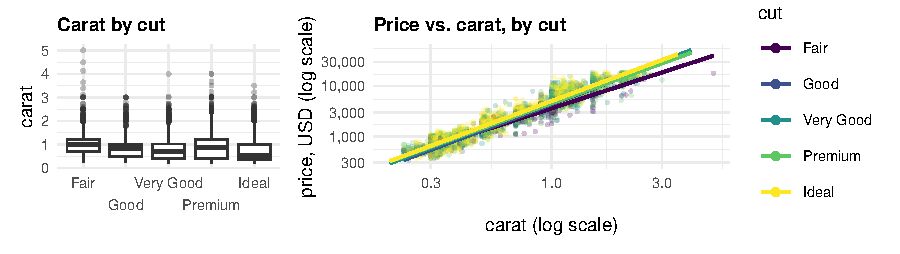
\includegraphics[width=0.95\linewidth,height=3.8cm,keepaspectratio]{figures/eda_diamonds_cut_carat.pdf}
    \end{center}
    \footnotesize
    \begin{itemize}
        \item Left: Ideal stones are mostly small (median 0.54 carat) and Fair stones large (median 1.00 carat)
        \item Right: within every cut, price rises steeply with carat; at exactly 1 carat, Fair costs \$4,130 on average ($n=166$) and Ideal \$5,547 ($n=208$)
    \end{itemize}
\end{frame}

\begin{frame}{The EDA workflow}
    \centering
    \begin{tikzpicture}[
        stage/.style={draw=airforceblue, fill=airforceblue!15, rounded corners=2pt, minimum height=0.9cm, text width=0.15\linewidth, align=center, font=\scriptsize\bfseries},
        note/.style={text width=0.15\linewidth, align=center, font=\scriptsize},
        flow/.style={-{Latex[length=1.8mm]}, thick, draw=airforceblue}]
        \node[stage] (a) {First look};
        \node[stage, right=0.025\linewidth of a] (b) {One variable};
        \node[stage, right=0.025\linewidth of b] (c) {Two variables};
        \node[stage, right=0.025\linewidth of c] (d) {Many variables};
        \node[stage, right=0.025\linewidth of d] (e) {Decision};
        \node[note, below=1mm of a] {size, types, missing counts};
        \node[note, below=1mm of b] {centre, spread, shape};
        \node[note, below=1mm of c] {association, groups};
        \node[note, below=1mm of d] {structure, redundancy};
        \node[note, below=1mm of e] {rule, model, or more data?};
        \foreach \s/\t in {a/b, b/c, c/d, d/e} \draw[flow] (\s) -- (\t);
        \draw[flow, dashed] (e.north) -- ++(0,0.6) coordinate (r) -| (a.north);
        \node[above, font=\scriptsize] at (c |- r) {new questions};
    \end{tikzpicture}
    \svspace{1em}
    \begin{itemize}
        \item Each stage raises questions for the next, so EDA is iterative rather than a fixed pipeline
        \item The decision at the end is not always ``fit a model'': it may be to collect more data, apply a simple rule rather than a complex ML algorithm, or report the summary
    \end{itemize}
\end{frame}

\begin{frame}{First look at a dataset}
    \begin{itemize}
        \item Size and types: number of rows and columns and the type of each variable
        \item Missing values: count them per variable; take necessary actions in case of any missing values
        \item Duplicate rows and impossible values, such as negative ages or zero dimensions
        % \item Titanic (891 passengers): age is missing for 177 passengers, deck for 688, and port of embarkation for 2
    \end{itemize}
\end{frame}


\section{One Variable at a Time}


\begin{frame}{Location: mean, median, trimmed mean, mode}
    Observations $x_1,\dots,x_n$ of one numeric variable.
    \svspace{0.5em}
    \begin{itemize}
        \item \textbf{Mean} $\bar{x}=\frac{1}{n}\sum_{i=1}^{n}x_i$: uses every value, so extreme values pull it
        \item \textbf{Median}: the middle value of the sorted data, with half of the observations on each side; extreme values do not move it, so it is the better measure of centre for skewed data such as prices, incomes, or waiting times
        \item \textbf{Trimmed mean}: the mean after discarding a fixed share (say 10\%) of observations from each tail
        \item \textbf{Mode}: the most frequent value
    \end{itemize}
\end{frame}


\begin{frame}{Spread and shape}
    \begin{itemize}
        \item \textbf{Standard deviation}: $s=\sqrt{\frac{1}{n-1}\sum_{i=1}^{n}(x_i-\bar{x})^2}$: typical distance from the mean; sensitive to extreme values
        \item \textbf{Interquartile range}: third quartile minus first quartile, $\mathrm{IQR}=Q_3-Q_1$: width of the middle 50\% of the data; robust to extreme values
        \item \textbf{Skewness}: $g_1=\frac{1}{n}\sum_{i=1}^{n}\bigl(\frac{x_i-\bar{x}}{s}\bigr)^{3}$: positive for a long right tail, negative for a long left tail, near zero for a symmetric distribution
        \item \textbf{Kurtosis}: $g_2=\frac{1}{n}\sum_{i=1}^{n}\bigl(\frac{x_i-\bar{x}}{s}\bigr)^{4}-3$: positive when the tails are heavier than those of a normal distribution
    \end{itemize}
\end{frame}


\begin{frame}{Summary statistics in practice: diamonds}
    \begin{columns}[T]
        \begin{column}{0.43\textwidth}
            \footnotesize
            \setlength{\tabcolsep}{3pt}
            \begin{tabular}{@{}lrr@{}}
                \toprule
                & price (USD) & carat \\
                \midrule
                Mean & 3,933 & 0.80 \\
                10\% trimmed & 3,159 & 0.73 \\
                Median & 2,401 & 0.70 \\
                Std. dev. & 3,989 & 0.47 \\
                IQR & 4,374 & 0.64 \\
                MAD & 1,670 & 0.32 \\
                Skewness & 1.62 & 1.12 \\
                Ex. kurtosis & 2.18 & 1.26 \\
                \bottomrule
            \end{tabular}
        \end{column}
        \begin{column}{0.50\textwidth}
            \small
            \begin{itemize}
                \item The mean price is 64\% above the median: a few expensive stones pull the mean up, while the median describes a typical stone
                \item Skewness of 1.62 confirms a long right tail; mean $>$ median and positive skewness go together
            \end{itemize}
        \end{column}
    \end{columns}
\end{frame}


\begin{frame}{Histograms and density estimates}
    \begin{center}
        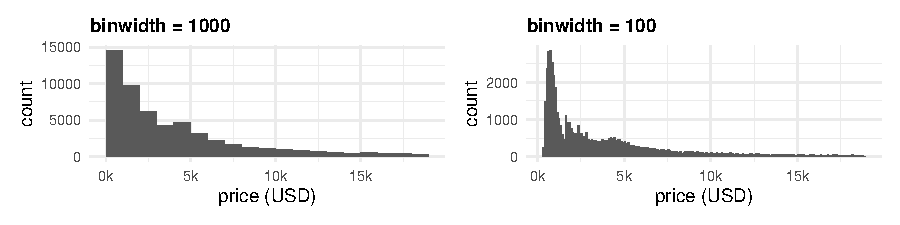
\includegraphics[width=0.95\linewidth,height=3.4cm,keepaspectratio]{figures/eda_diamonds_hist_density.pdf}
    \end{center}
    \footnotesize
    \begin{itemize}
        \item \textbf{Histogram:} counts in equal-width bins; try several widths (wide bins hide structure, narrow bins add noise); read peaks, gaps, and spikes
        \begin{itemize}
            \item At width 100 the count falls to 463 in \$1,500--1,599 and jumps to 1,115 in the next bin, a jump that width 1000 hides
            \item Use with hundreds of observations or more; for small samples use a dot or strip plot
        \end{itemize}
    \end{itemize}
\end{frame}


\begin{frame}{Boxplot, violin plot, and ECDF}
    \begin{center}
        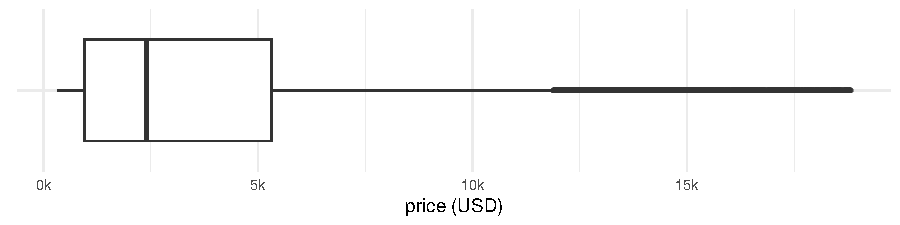
\includegraphics[width=0.95\linewidth,height=3.4cm,keepaspectratio]{figures/eda_diamonds_box_violin_ecdf.pdf}
    \end{center}
    \footnotesize
    \begin{itemize}
        \item \textbf{Boxplot:} box from $Q_1$ to $Q_3$ with the median line; whiskers reach the furthest points within $1.5\times\mathrm{IQR}$; points beyond are flagged (3,540 stones, 6.6\%, all expensive)
        \begin{itemize}
            \item Use to compare many groups side by side; it cannot show several peaks
        \end{itemize}
    \end{itemize}
\end{frame}


\begin{frame}{Categorical variables: frequencies and bar charts}
    \begin{center}
        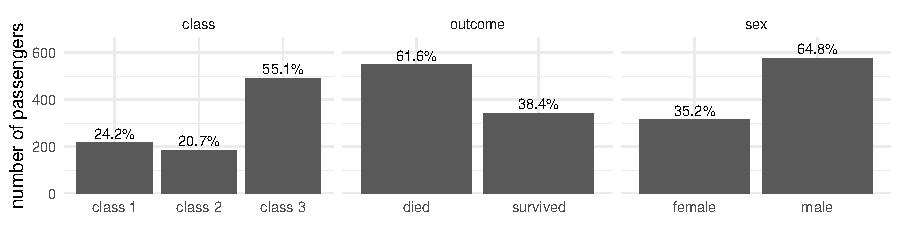
\includegraphics[width=0.95\linewidth,height=3.4cm,keepaspectratio]{figures/eda_titanic_bars.pdf}
    \end{center}
    \footnotesize
    \begin{itemize}
        \item A frequency table lists the count and share of each level, and the bar chart is its picture
        \item Titanic, 891 passengers: 61.6\% died and 38.4\% survived; 55.1\% travelled third class; 64.8\% were male
        \item Imbalance matters: predicting ``died'' for everyone is already 61.6\% accurate, a baseline any model must beat
        \item Order nominal levels by frequency and ordinal ones naturally
    \end{itemize}
\end{frame}


\section{Data Quality}

\begin{frame}{Missing values: count first, then decide}
    \begin{center}
    \footnotesize
    \begin{tabular}{llrr}
        \toprule
        Dataset & Variable & Missing & Share \\
        \midrule
        Titanic (891 rows) & age & 177 & 19.9\% \\
        & deck & 688 & 77.2\% \\
        & embarked & 2 & 0.2\% \\
        California housing (20,640) & total\_bedrooms & 207 & 1.0\% \\
        \bottomrule
    \end{tabular}
    \end{center}
    \footnotesize
    \begin{itemize}
        \item Count the missing values per variable: 2 missing values (embarked) call for a different response than 77\% (deck)
        \item Ask why: Titanic age is missing for 27.7\% of third-class but 6.0\% of second-class passengers, so not at random; total\_bedrooms is missing at 0.8--1.1\% in each large ocean-proximity group, no visible pattern
        \item Missing values can hide as codes (99, $-1$, 0), common in survey microdata; check value counts
        \item If any are present, judge whether action is required and take the necessary steps (preprocessing lecture)
    \end{itemize}
\end{frame}

\begin{frame}{Detecting outliers}
    \begin{center}
        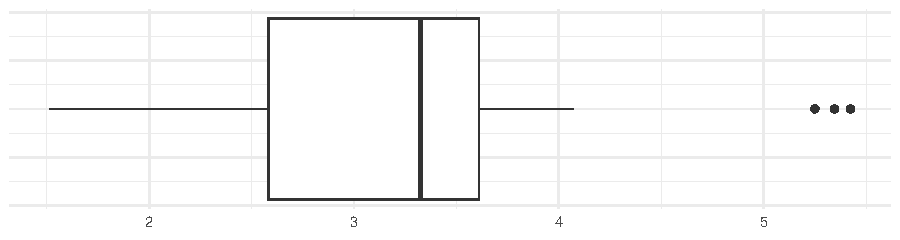
\includegraphics[width=0.95\linewidth,height=3.6cm,keepaspectratio]{figures/eda_mtcars_wt_boxplot.pdf}
    \end{center}
    \footnotesize
    \begin{itemize}
        \item \textbf{$1.5\times\mathrm{IQR}$ rule:} flag values below $Q_1-1.5\,\mathrm{IQR}$ or above $Q_3+1.5\,\mathrm{IQR}$
        \item \textbf{$z$-score:} $z_i=(x_i-\bar{x})/s$, flag $\lvert z_i\rvert>3$; the mean and SD are pulled by the outliers themselves, which can mask them
        \item \textbf{Modified $z$-score:} $M_i=0.6745\,(x_i-\tilde{x})/\mathrm{MAD}$, flag $\lvert M_i\rvert>3.5$; robust, but on skewed data it flags the long tail
    \end{itemize}
\end{frame}


\section{Two Variables}

\begin{frame}{Two numeric variables: scatter plots}
    \begin{center}
        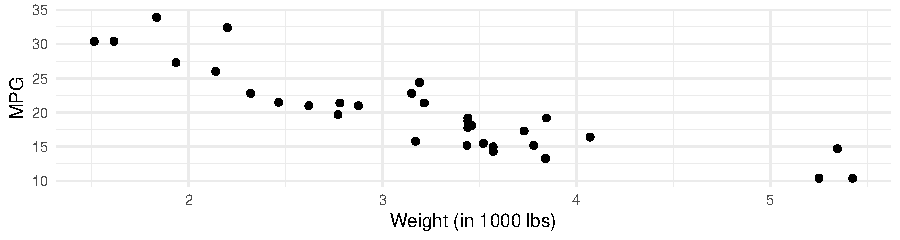
\includegraphics[width=0.95\linewidth,height=3.6cm,keepaspectratio]{figures/eda_mtcars-scatter.pdf}
    \end{center}
    \footnotesize
    \begin{itemize}
        \item A scatter plot puts each observation at $(x,y)$
        \item The overall shape of the plot can tell us whether there is any association between the two variables
        \item The correlation coefficeint is a numeric measure that quantifies the linear relationship between the two variables
    \end{itemize}
\end{frame}


\begin{frame}{Numeric variable across groups}
    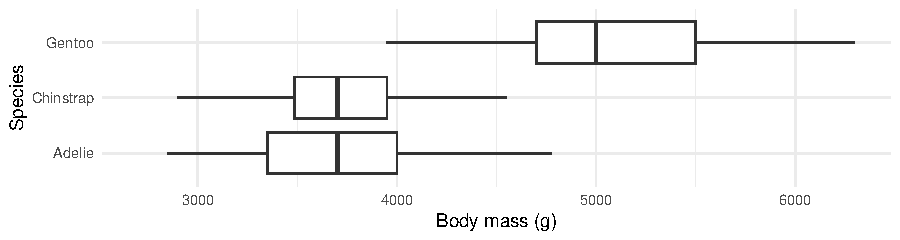
\includegraphics[width=0.95\linewidth,height=3.6cm,keepaspectratio]{figures/eda_penguins_mass_species.pdf}
    \footnotesize
    \begin{itemize}
        \item Mean body mass: Adelie 3,701 g, Chinstrap 3,733 g, Gentoo 5,076 g; the first two are nearly equal, Gentoo is about 1.4 kg heavier
        \item Mean $\pm$ 1.96 SE intervals (about $\pm$73, $\pm$91, $\pm$89 g) overlap for Adelie and Chinstrap; ANOVA gives $F(2,339)=343.6$, $\eta^2=0.67$: species explains 67\% of the variance
        \item Choose the plot by the question
        \begin{itemize}
            \item Boxplot with points: many groups; ridgeline: shape; mean and interval: means only
        \end{itemize}
    \end{itemize}
\end{frame}

\begin{frame}{Two categorical variables}
    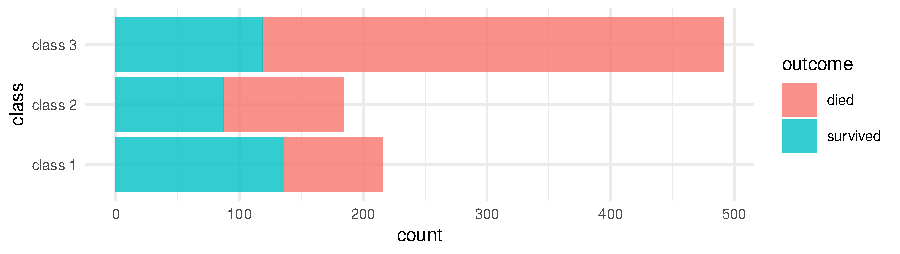
\includegraphics[width=0.95\linewidth,height=3.8cm,keepaspectratio]{figures/eda_titanic_stacked-barplot.pdf}
    \footnotesize
    \begin{itemize}
        \item Above is a stacked barplot
        \item It shows the proportion of survived passengers among different passenger classes in the Titanic
    \end{itemize}
\end{frame}

\section{Many Variables}


\begin{frame}{Correlation heatmap and multicollinearity}
    \begin{columns}[T]
        \begin{column}{0.46\textwidth}
            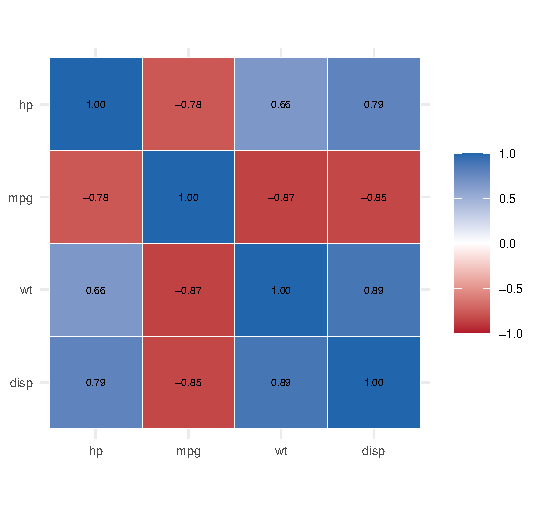
\includegraphics[width=\linewidth,height=5.3cm,keepaspectratio]{figures/eda_mtcars_corr.pdf}
        \end{column}
        \begin{column}{0.50\textwidth}
            \footnotesize
            \begin{itemize}
                \item Heatmap: a tile per pair, diverging colours centred at zero; clustering the order puts related variables in blocks
                \item mtcars: mpg vs. weight $-0.87$, cylinders $-0.85$, displacement $-0.85$; displacement vs. cylinders 0.90, weight 0.89
                \item Multicollinearity: overlapping predictors; $\mathrm{VIF}_j=1/(1-R_j^2)$, $R_j^2$ from regressing predictor $j$ on the others; cyl 6.7, disp 10.4, hp 3.4, wt 4.8 (concern above about 5--10)
                \item Shows pairwise linear association only
            \end{itemize}
        \end{column}
    \end{columns}
\end{frame}

\begin{frame}{More dimensions: colour, shape, facets, parallel coordinates}
    \begin{center}
        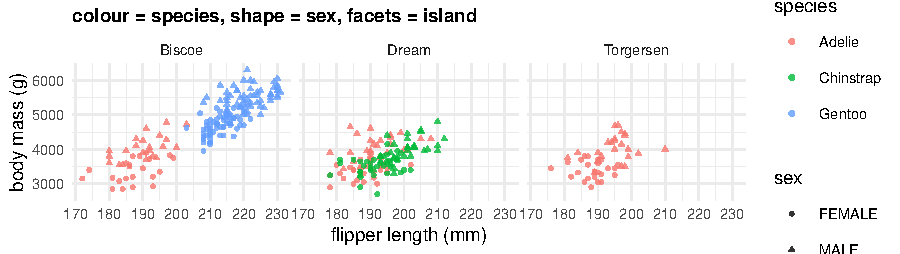
\includegraphics[width=0.95\linewidth,height=3.8cm,keepaspectratio]{figures/eda_penguins_encodings.pdf}
    \end{center}
    \footnotesize
    \begin{itemize}
        \item Extra variables can be encoded by colour (categorical), size or a colour gradient (numeric), shape, or faceting into small multiples with shared scales; keep to three or four variables per plot
        \item Facets by island reveal structure: Gentoo lives only on Biscoe and Chinstrap only on Dream, while Adelie is on all three, so island and species are entangled
        \item Parallel coordinates draw one line per observation across standardised variables; species form bands (Gentoo: shallow bills, long flippers, high mass), but many lines overlap
    \end{itemize}
\end{frame}
